\documentclass[runningheads]{llncs}

\usepackage{graphicx}
\usepackage{url}
\usepackage{natbib}
\usepackage{lscape}
\usepackage{subfigure}
\usepackage{algorithm}
\usepackage{algorithmic}
\usepackage{setspace}
\usepackage{color}
\usepackage{tikz}
\usepackage{amssymb}
\usepackage{amsmath}


\urldef{\mailsg}\path|{rax222}@gmu.edu|
\newcommand{\keywords}[1]{\par\addvspace\baselineskip
\noindent\keywordname\enspace\ignorespaces#1}

\begin{document}


\mainmatter

\title{Simulating Financial Markets using MASON Framework\thanks{Prepared for the 2nd World Congress on Social Simulation, GMU, Fairfax, 14--17 July, 2008.}}

\titlerunning{Financial Markets using MASON}
\authorrunning{R. Axtell et al.}

\author{Robert Axtell$^{a}$ \and CSS 739 Class Project Team}


\institute{
4400 University Drive, Fairfax VA 22030 \\
\mailss \\
\url{http://www.si.edu}}


\institute{$^{a}$Center for Social Complexity, George Mason University, USA \\
\mailsg}

\date{\today}
\maketitle
\begin{abstract}
AAA
\end{abstract}

\keywords{Agent-based Modeling, Computational Social Science, Financial Markets}

\section{Motivation and Objectives}


\section{Platform Architecture}

\begin{figure}[htb]
\centering
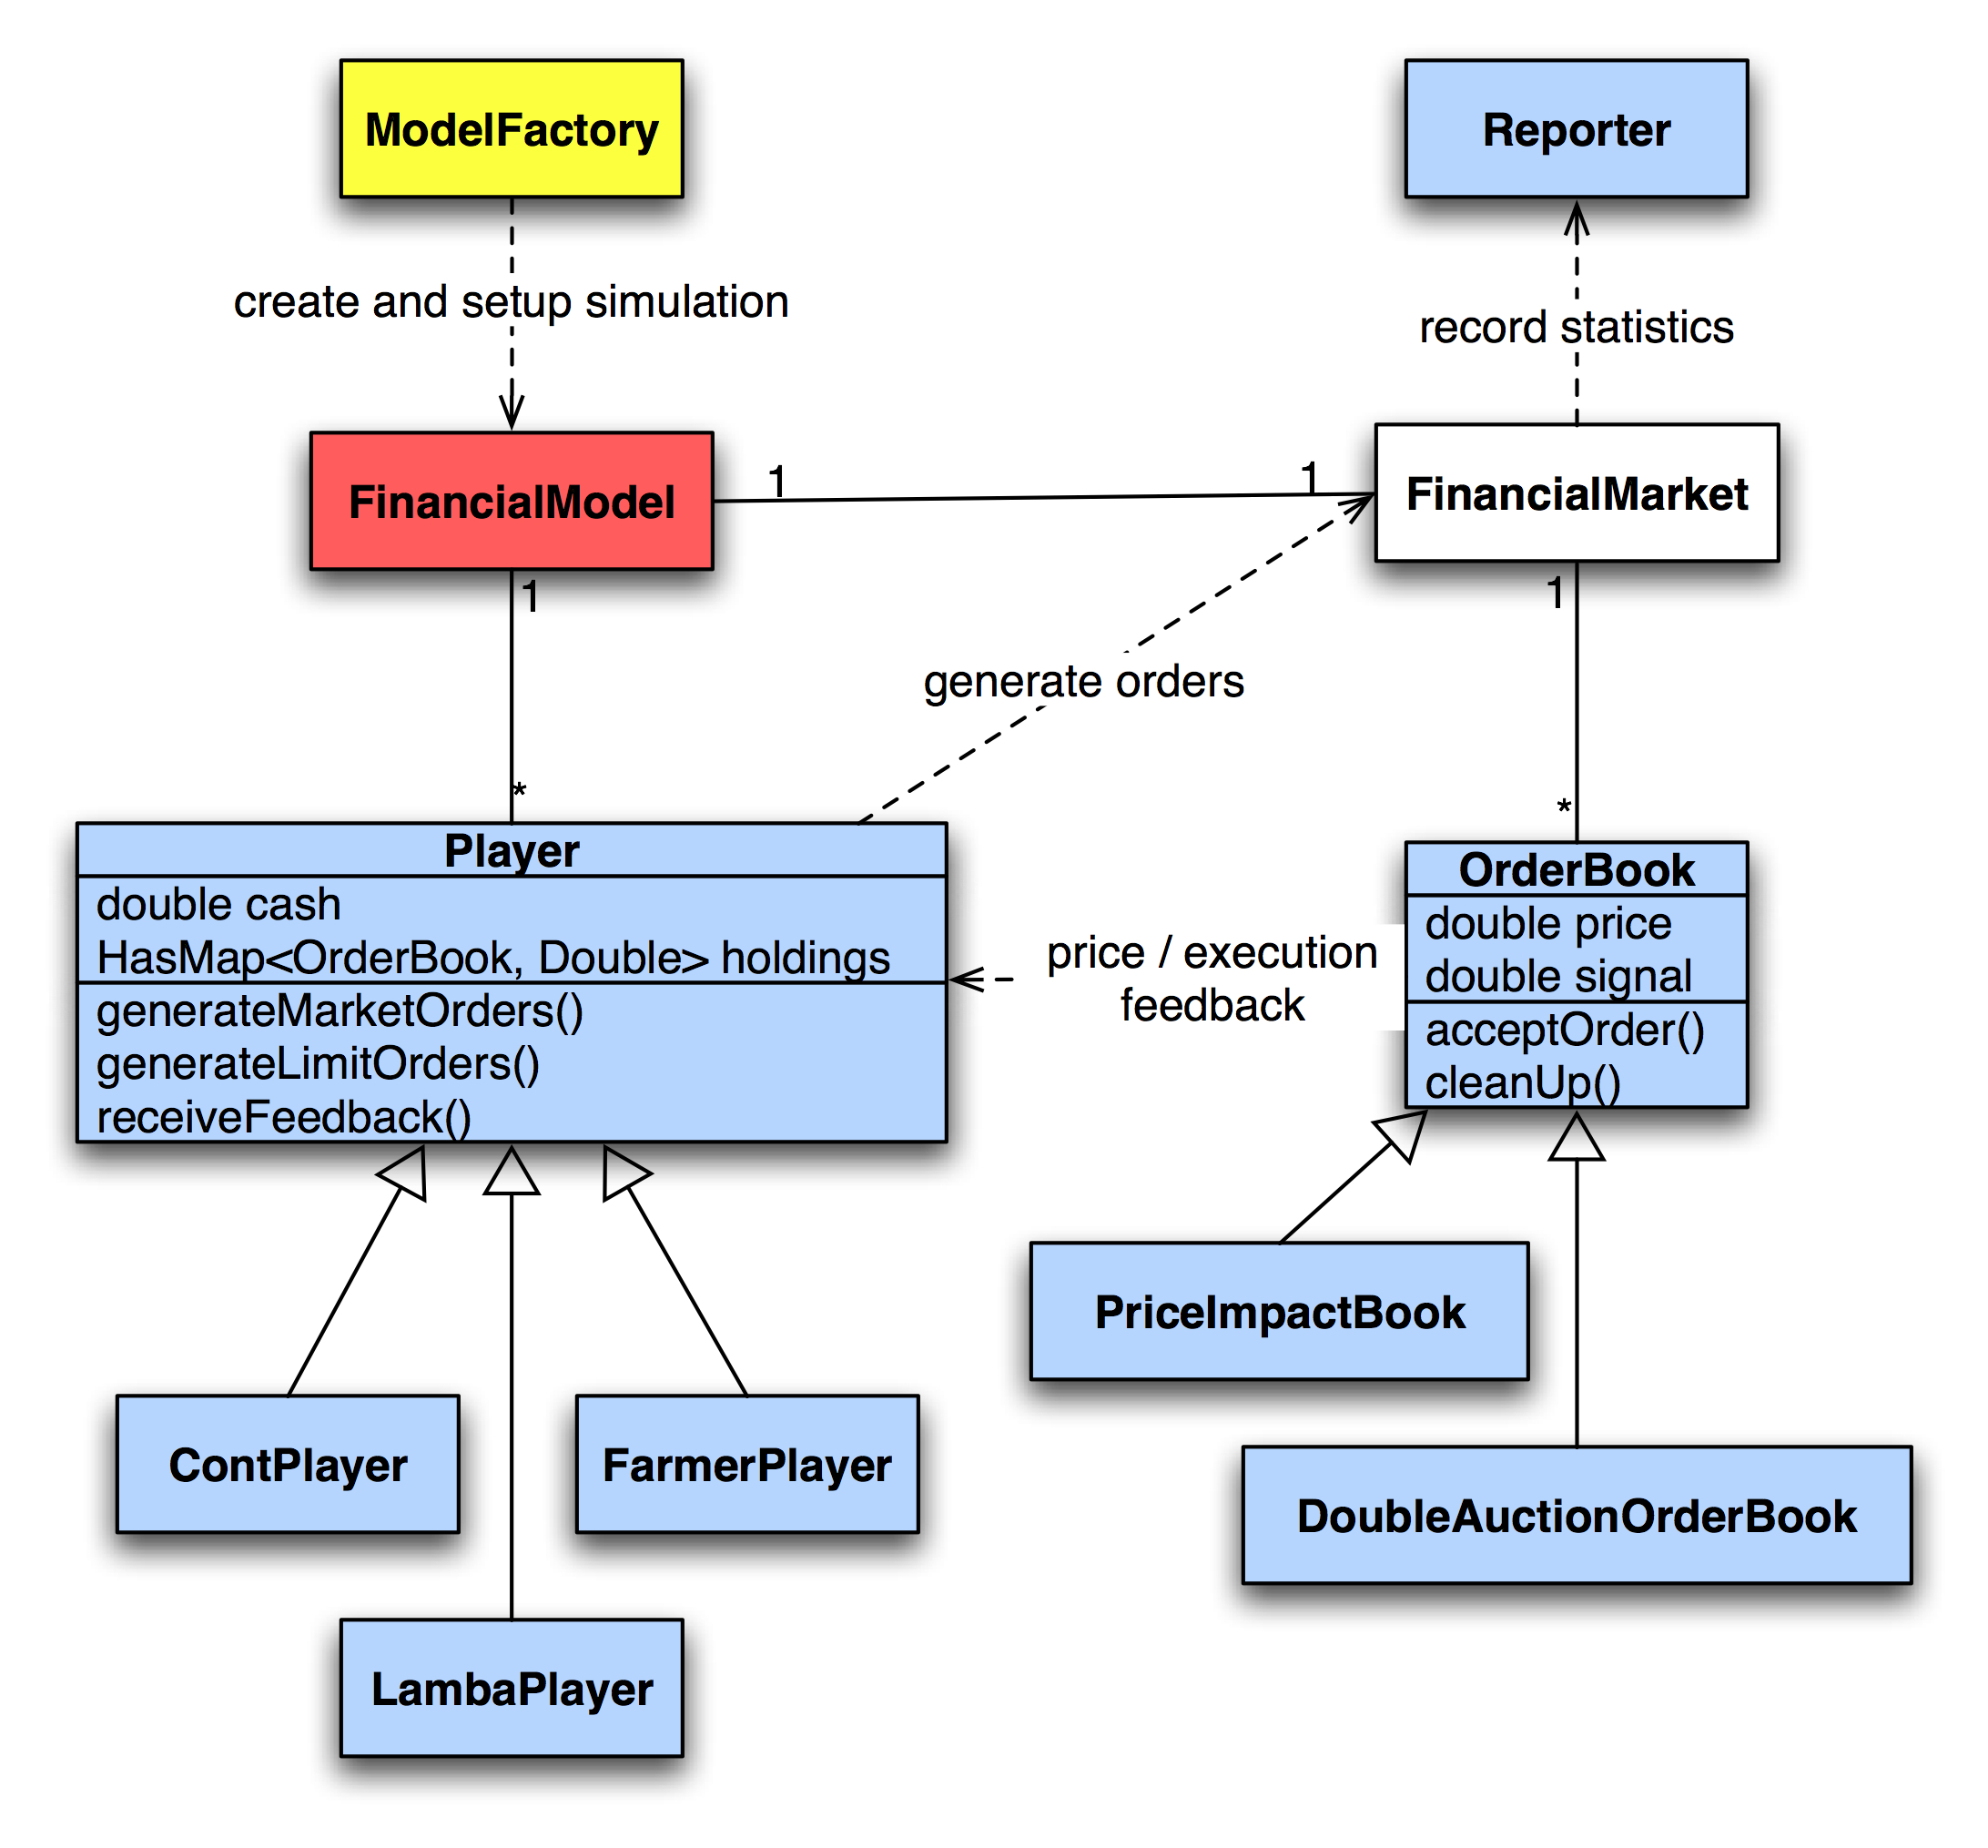
\includegraphics[width=1.0\textwidth]{../graphics/masterClassDiagram.jpg}
\caption{High-level UML class diagram of the main components and relations in the FinancialMarketModel, including the main attributes of Players and OrderBooks. Agent classes (light blue) inherit from the MASON \texttt{Steppable} interface while the master class is implementation of MASON's \texttt{SimState}.}
\label{fig:general_uml}
\end{figure}

\begin{figure}[htbp]
  \begin{center}
   \mbox{
      \subfigure[Ask and bid prices.]{\scalebox{0.5}{\quad \quad 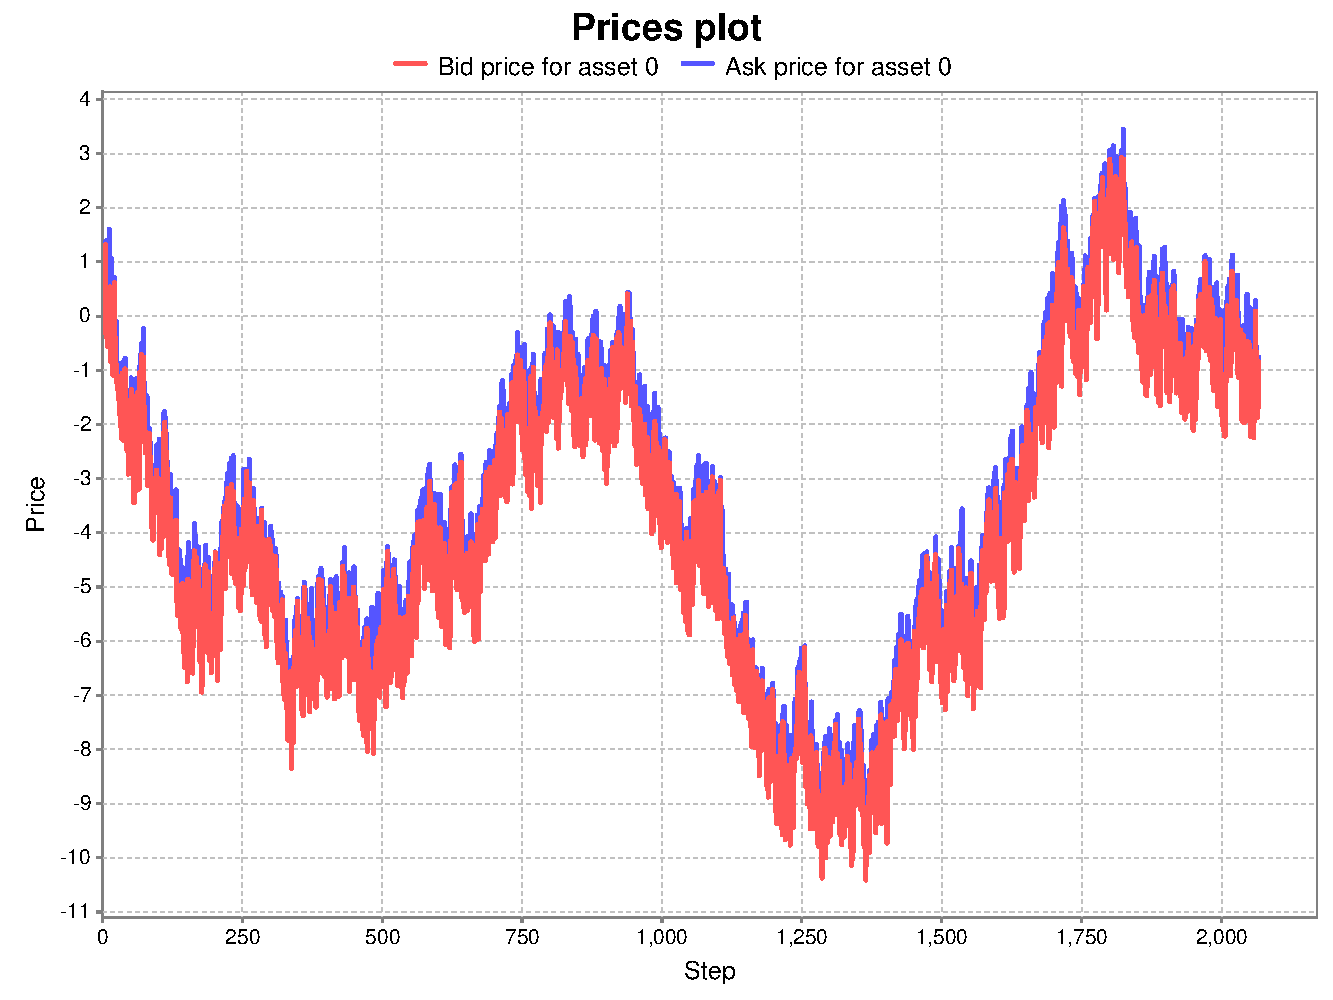
\includegraphics[width=0.9\textwidth,height=0.8\textwidth]{../graphics/pricesPlot.pdf}}} \quad
      \subfigure[Raw and absolute returns.]{\scalebox{0.5}{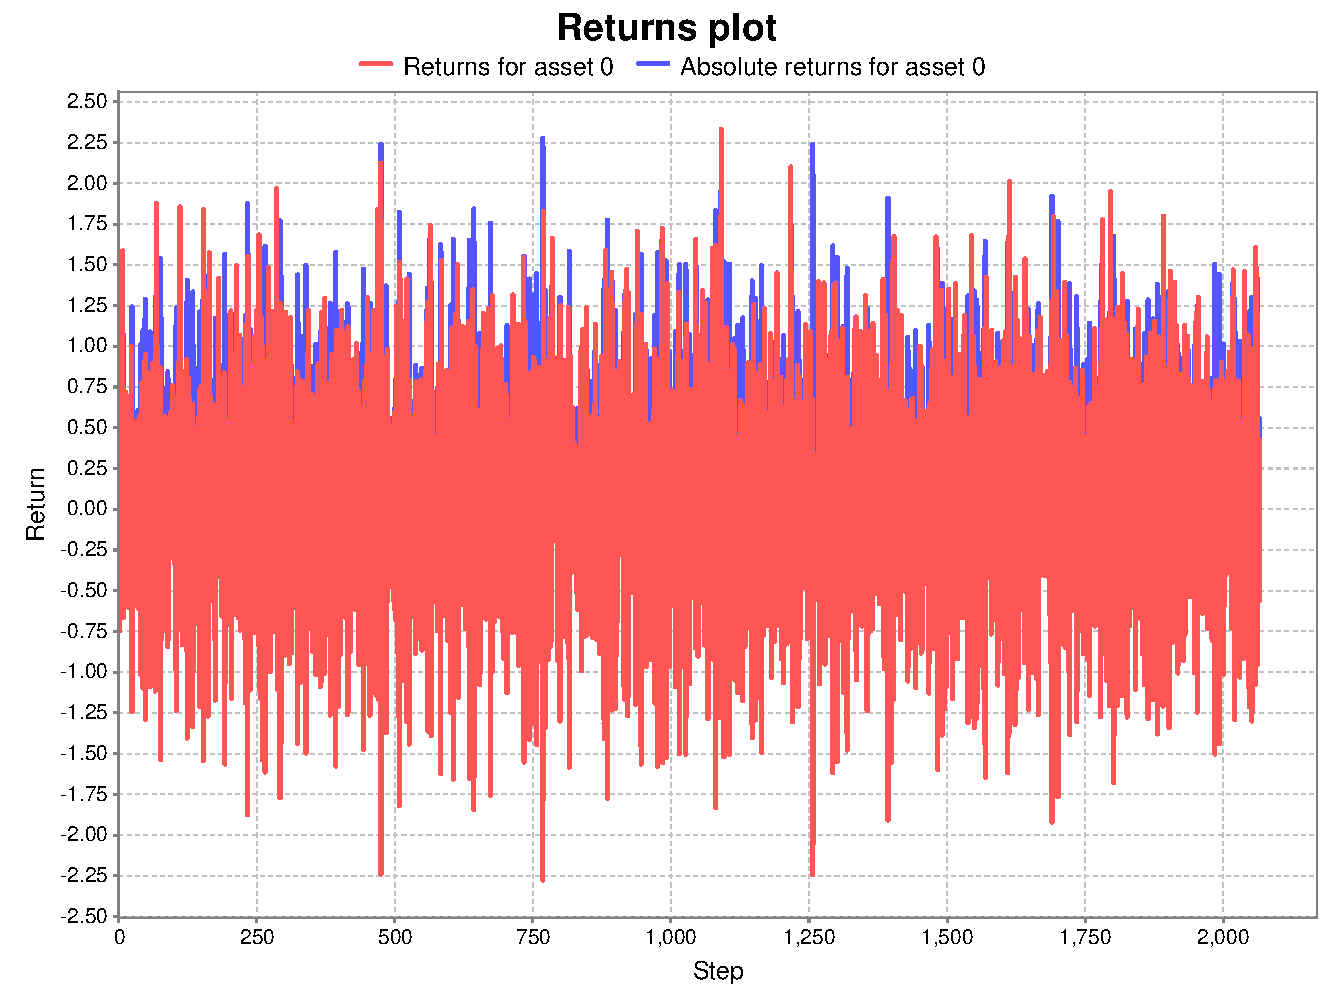
\includegraphics[width=1.00\textwidth]{../graphics/returnPlot.pdf}}}
      }
    \mbox{
      \subfigure[Orderbook shape.]{\scalebox{0.5}{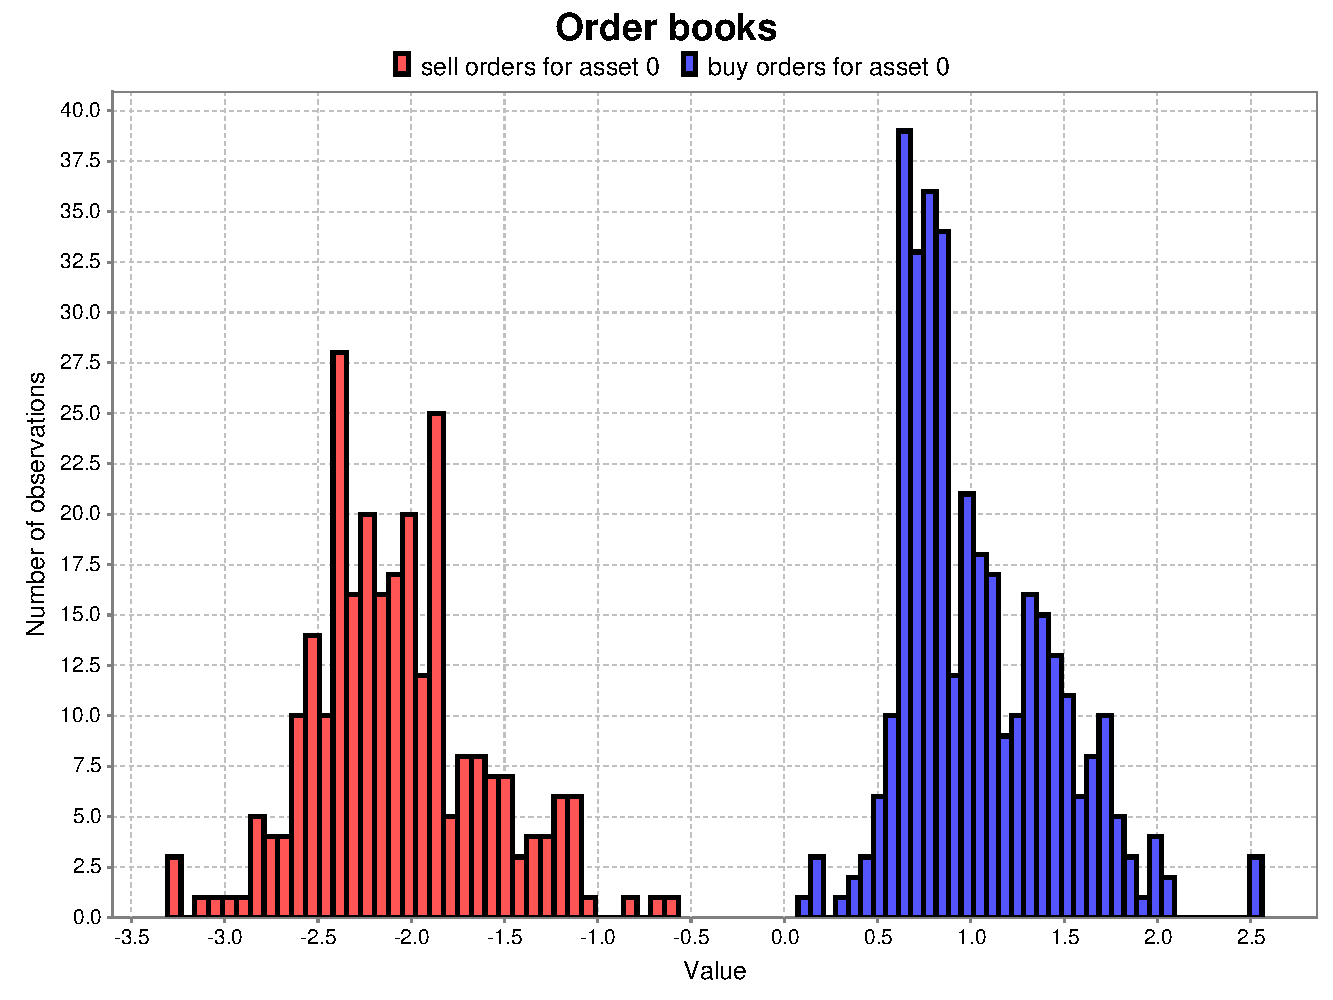
\includegraphics[width=1.00\textwidth]{../graphics/orderbooks.pdf}}} \quad
      \subfigure[Trade volumes.]{\scalebox{0.5}{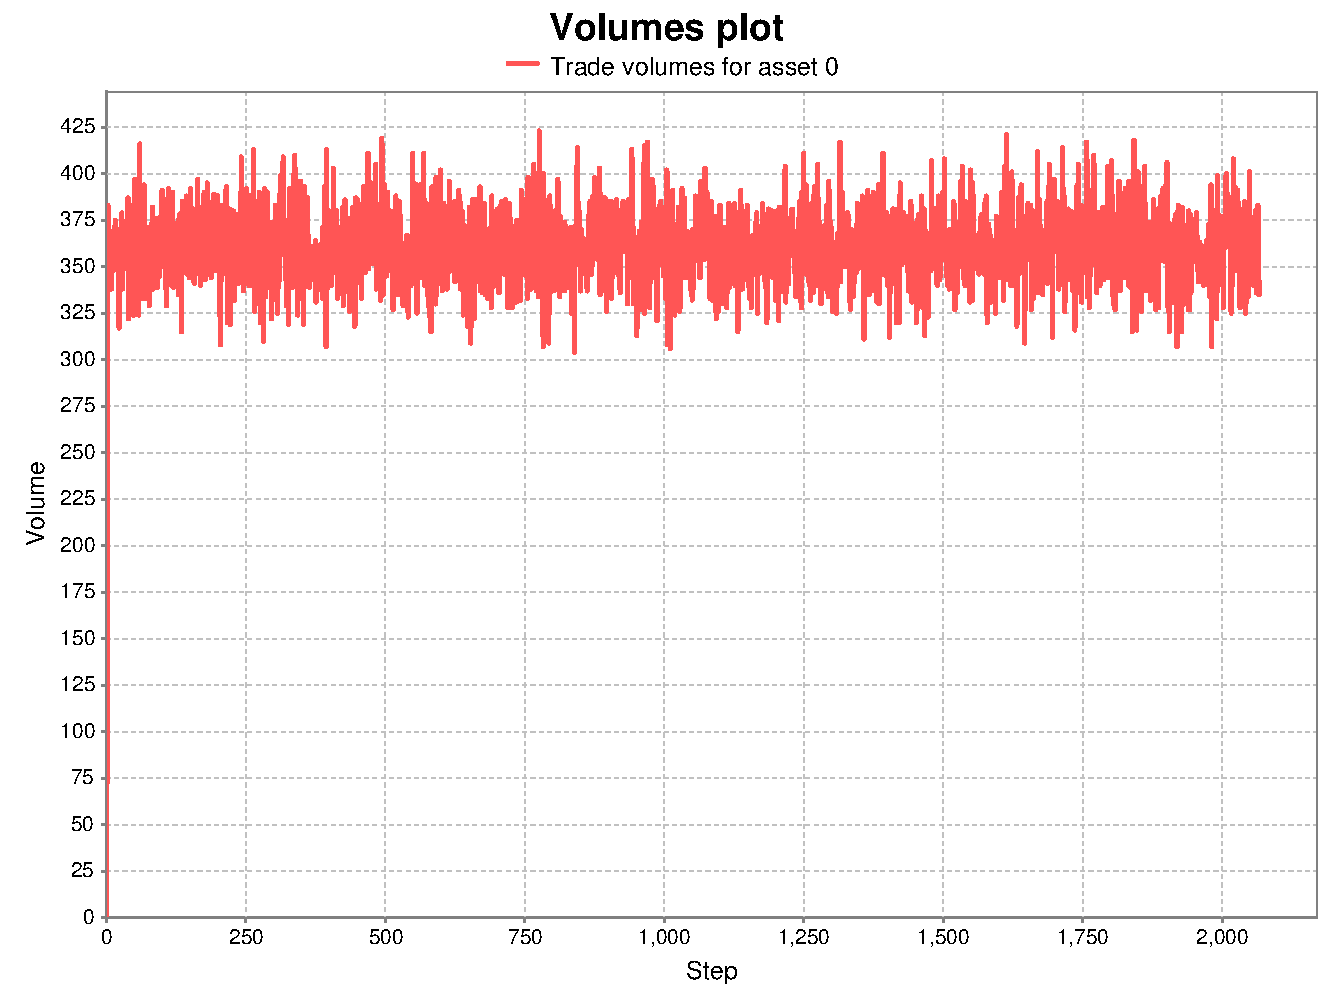
\includegraphics[width=1.00\textwidth]{../graphics/volumesPlot.pdf}}}
      }
    \mbox{
      \subfigure[Returns histogram.]{\scalebox{0.5}{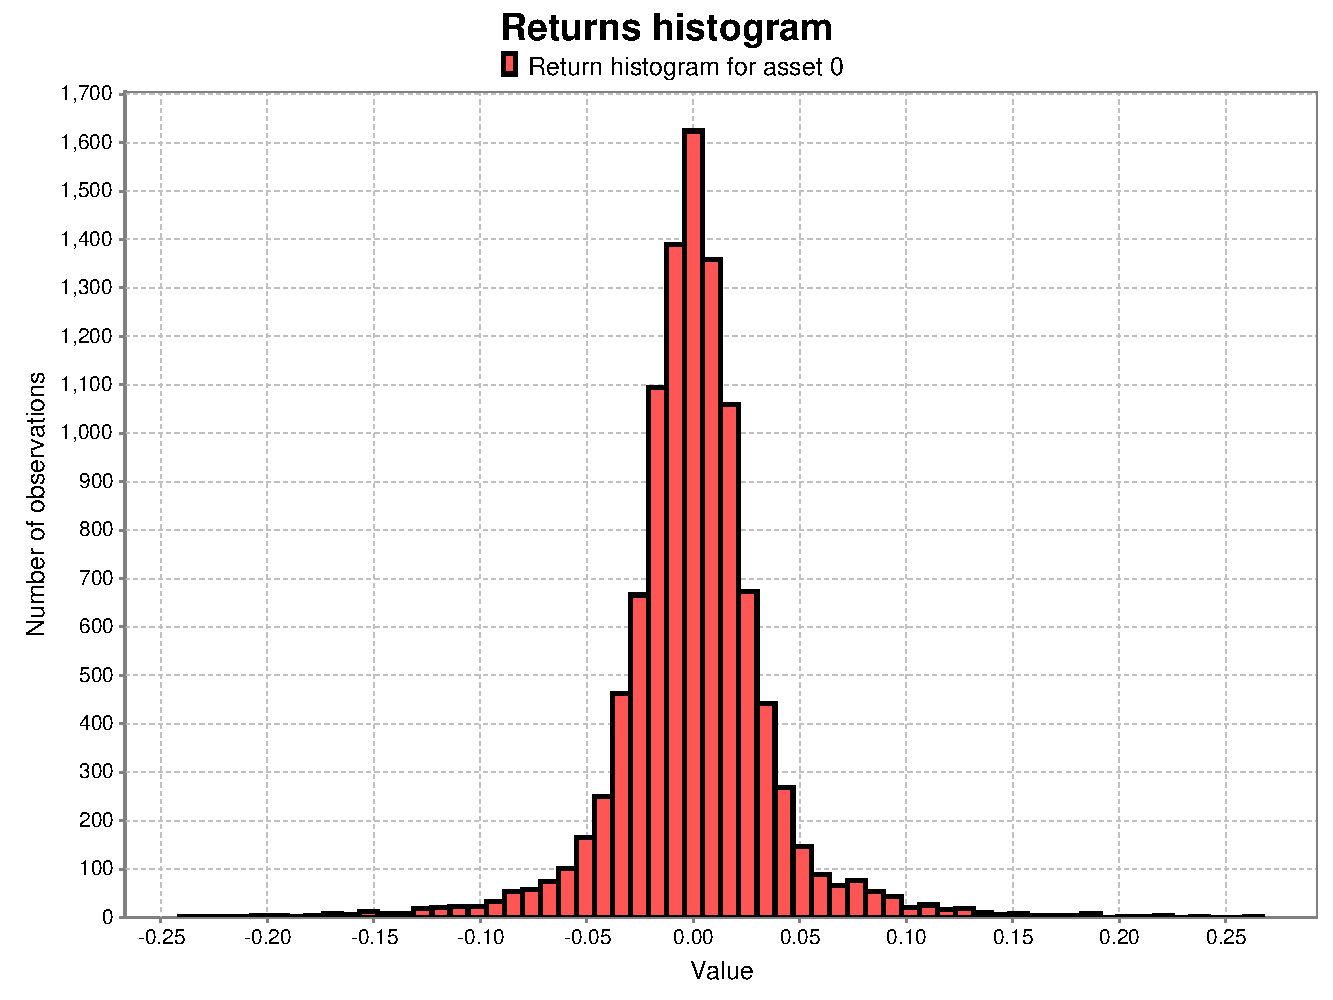
\includegraphics[width=1.00\textwidth]{../graphics/returnsHistogram.pdf}}} \quad
      \subfigure[Autocorrelation of returns.]{\scalebox{0.5}{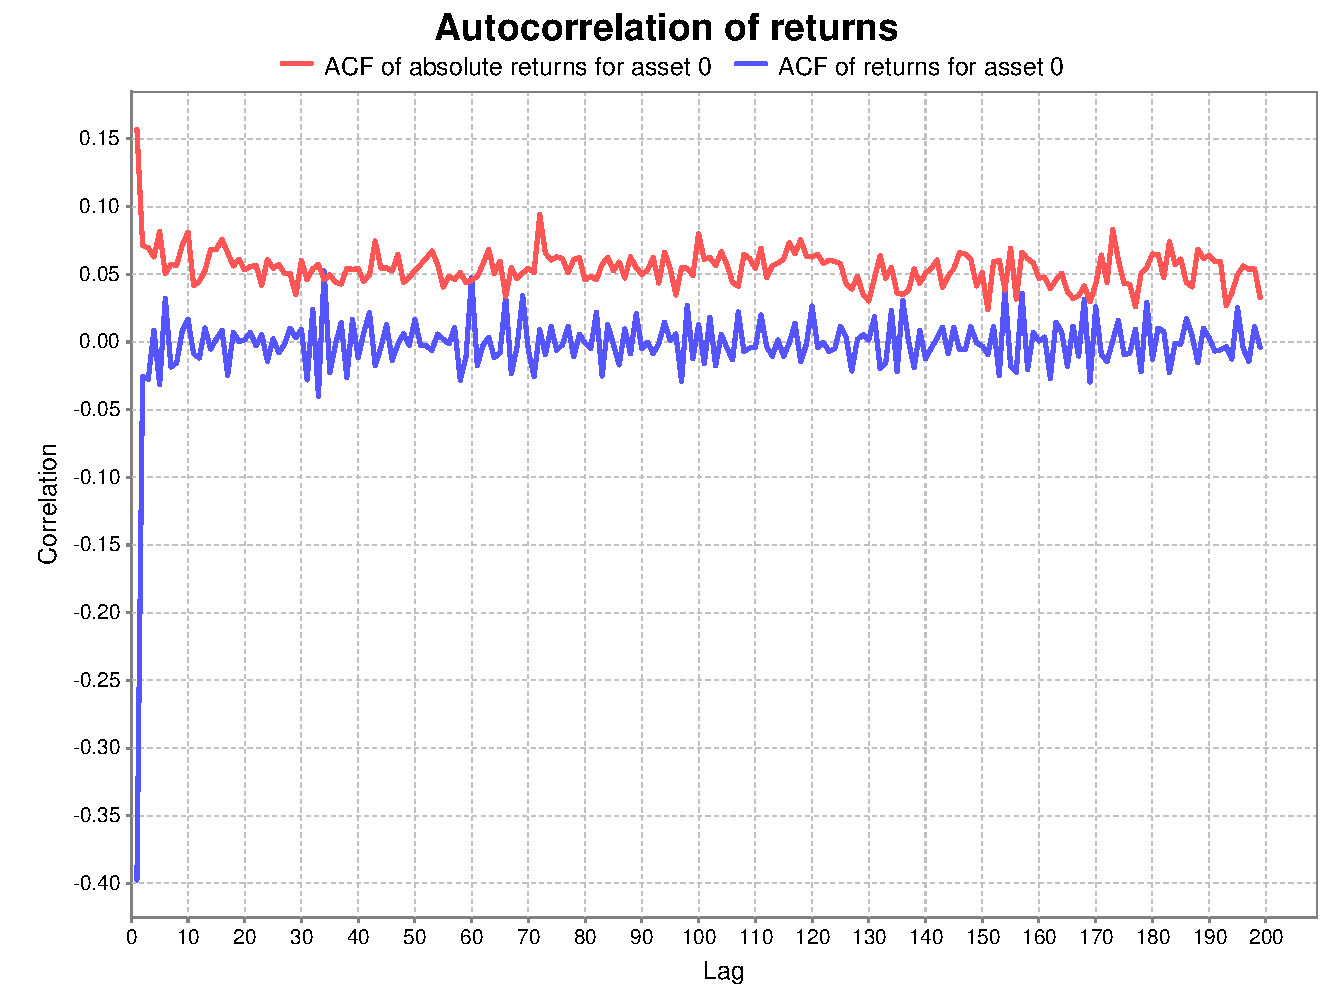
\includegraphics[width=1.00\textwidth]{../graphics/acfReturns.pdf}}}
      }
    \caption{Examples of outputs and statistics from a single run of the FinancialModel simulation for default Farmer's parametrization.}
    \label{fig:sampleDynamics}
  \end{center}
\end{figure}


\section{Verification of Correctness}

\section{Overview of Implemented Models}

\begin{itemize}
	\item \cite{farmer2003}
	\item \cite{lamba2007}
	\item \cite{westerhoff2004}
	\item \cite{cont2006}
\end{itemize}

\bibliographystyle{plainnat}
\bibliography{master}

\end{document}

%%%%%%%%%%%%%%%%%%%%%%%%%%%%%%%%%%%%%%%%%%%%%%%%%%%%%%%%%%%%%%%%%%%%%%
%% The end.
%%%%%%%%%%%%%%%%%%%%%%%%%%%%%%%%%%%%%%%%%%%%%%%%%%%%%%%%%%%%%%%%%%%%%% 
